\hypertarget{functional-programming-1}{%
\section{Functional Programming 1}\label{functional-programming-1}}

\hypertarget{correctness}{%
\subsection{Correctness}\label{correctness}}

A program should be correct with respect to its specification. e.g.~a
program that computes the sine perfectly well but should compute the
root is clearly not correct.

One can know wether the program is correct

\begin{itemize}
\tightlist
\item
  by testing

  \begin{itemize}
  \tightlist
  \item
    choose particular input•determine correct result for that input
    using test oracle
  \item
    run program under test on the chosen input
  \item
    compare obtained and correct result
  \end{itemize}
\item
  by proving

  \begin{itemize}
  \tightlist
  \item
    no particular input
  \item
    no execution of the program
  \item
    instead apply mathematical rules to program and specification
  \item
    with a finite number of steps prove that something works for a
    infinite number of values
  \end{itemize}
\end{itemize}

\hypertarget{referential-transparency}{%
\subsection{Referential Transparency}\label{referential-transparency}}

\hypertarget{formal-proof}{%
\subsubsection{Formal proof}\label{formal-proof}}

\begin{figure}[H]
\centering
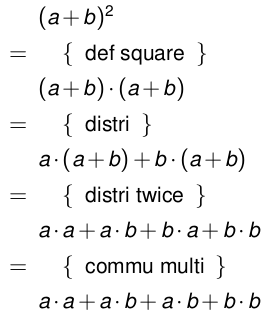
\includegraphics[width=0.25\textwidth]{figures/formalproof1.png}
\caption{Formal proof 1}
\end{figure}

\begin{figure}[H]
\centering
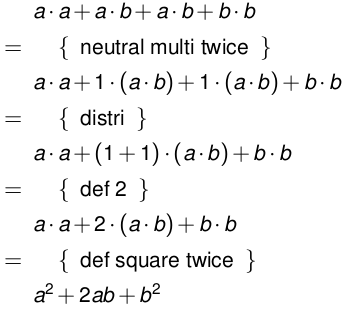
\includegraphics[width=0.25\textwidth]{figures/formalproof2.png}
\caption{Formal proof 2}
\end{figure}

\hypertarget{equality}{%
\subsubsection{Equality}\label{equality}}

\begin{figure}[H]
\centering
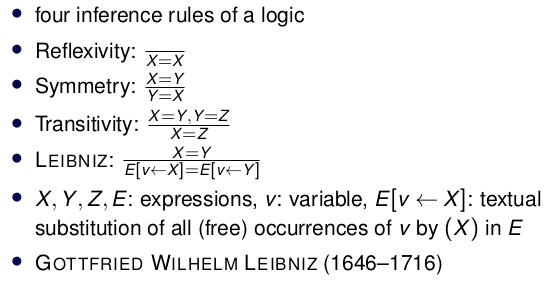
\includegraphics[width=0.5\textwidth]{figures/equality.png}
\caption{Equality}
\end{figure}

\begin{figure}[H]
\centering
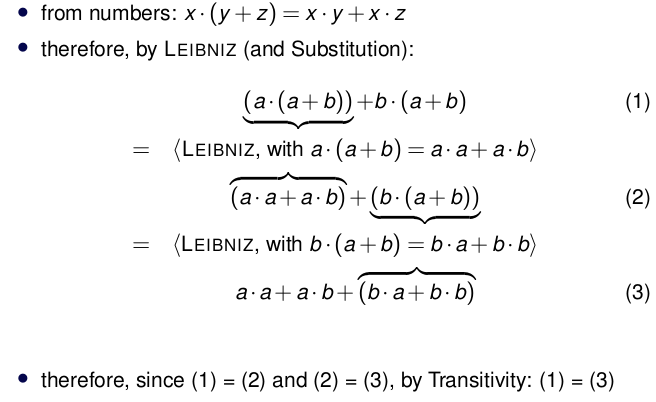
\includegraphics[width=0.5\textwidth]{figures/leibniz.png}
\caption{Example from Leibniz}
\end{figure}

\hypertarget{functional-program}{%
\subsubsection{Functional Program}\label{functional-program}}

\begin{itemize}
\item
  a functional program consists of

  \begin{enumerate}
  \def\labelenumi{\arabic{enumi}.}
  \tightlist
  \item
    a set of value and function declarations
  \item
    a single expression
  \end{enumerate}
\item
  functional programming is referentially transparent

  \begin{itemize}
  \tightlist
  \item
    values and functions are declared via equality
  \item
    equality then means mathematical equality (if using eager evaluation
    modulo termination)
  \end{itemize}
\item
  referential transparency employed for

  \begin{itemize}
  \tightlist
  \item
    program development, transformation, and proof
  \item
    evaluation
  \end{itemize}
\end{itemize}

\clearpage
\hypertarget{imperative-programming}{%
\subsection{Imperative Programming}\label{imperative-programming}}

\begin{itemize}
\tightlist
\item
  syntax: expressions + commands
\item
  semantics: values + environment + state
\item
  expressions are evaluated in the environment and current state,
  yielding a value
\item
  commands are executed in the environment and current state, yielding a
  new state
\item
  Example:

  \begin{itemize}
  \tightlist
  \item
    assignment command with variable v and expression E -\textgreater{}
    v := E
  \item
    E is evaluated in the environment and current state, yielding value
    t; then t is assigned to the storage cell denoted by v in the
    environment, thus yielding a new state
  \end{itemize}
\item
  proofs of imperative programs are well possible too, but are by far
  more complicated
\item
  possible using HOARE logic
\item
  HOARE triple, with P, Q predicates and C command:

  \begin{itemize}
  \tightlist
  \item
    \{P\} C \{Q\}
  \item
    means: if execution of C starts in a state satisfying P, and
    execution terminates, then the resulting state satisfies Q
  \end{itemize}
\item
  Example:

  \begin{itemize}
  \tightlist
  \item
    proof rule for assignment command v := E
  \item
    \{Q{[}v \textless{}- E{]}\} v := E \{Q\}
  \end{itemize}
\end{itemize}

\hypertarget{conclusion-on-imperative-vs.functional}{%
\subsection{Conclusion on Imperative
vs.~Functional}\label{conclusion-on-imperative-vs.functional}}

\textbf{imperative paradigm}

\begin{itemize}
\tightlist
\item
  syntax: expressions + commands
\item
  semantics: values + environment + state
\item
  expressions are evaluated in the environment and current state,
  yielding a value
\item
  commands are executed in the environment and current state, yielding a
  new state
\end{itemize}

\textbf{functional paradigm}

\begin{itemize}
\tightlist
\item
  syntax: expressions
\item
  semantics: values + environment
\item
  expressions are evaluated in the environment, yielding a value
\end{itemize}

\hypertarget{misuse-of-the-symbol-for-equality}{%
\subsubsection{Misuse of the Symbol for Equality
=}\label{misuse-of-the-symbol-for-equality}}

\begin{itemize}
\tightlist
\item
  assignment like x := x + 1 has not the slightest similarity to
  equality
\item
  it is pronounced ``x becomes (gets, receives) x + 1'' \ldots{}
\item
  \ldots{} but never ever ``x equals (is, is equal to) x + 1''
\item
  a different symbol like := or ← should be used instead
\item
  using the symbol for equality = to denote assignment is a horrendous
  design error of too many programming languages.
\end{itemize}

\hypertarget{evaluation}{%
\subsection{Evaluation}\label{evaluation}}

\begin{itemize}
\tightlist
\item
  strategies

  \begin{itemize}
  \tightlist
  \item
    innermost (call-by-value)
  \item
    outermost (call-by-name)
  \item
    \textbf{lazy (outermost + sharing)}
  \item
    reducible expression, or redex
  \item
    application of a function to its argument expressions
  \end{itemize}
\item
  Example: mult(x,y) = x * y

  \begin{itemize}
  \tightlist
  \item
    mult(1+2, 2+3) has three redexes

    \begin{itemize}
    \tightlist
    \item
      1+2, yielding mult(3,2+3)
    \item
      2+3, yielding mult(1+2,5)
    \item
      mult(1+2,2+3) yielding (1+2)*(2+3)
    \end{itemize}
  \end{itemize}
\end{itemize}

\hypertarget{innermost-evaluation}{%
\subsubsection{Innermost Evaluation}\label{innermost-evaluation}}

innermost redex first; if several, choose leftmost one first

mult (1+2,2+3)\\
= mult (3,2+3)\\
= mult (3,5)\\
= 3*5\\
= 15

\clearpage
\hypertarget{outermost-evaluation}{%
\subsubsection{Outermost Evaluation}\label{outermost-evaluation}}

outermost redex first; if several, choose leftmost one first

mult (1+2,2+3)\\
= (1+2) * (2+3)\\
= 3 * (2+3)\\
= 3 * 5\\
= 15

\hypertarget{lazy-evaluation}{%
\subsubsection{Lazy Evaluation}\label{lazy-evaluation}}

Argument expressions might be evaluated more than once if the
corresponding formal parameters occur several times in the body of the
function. Solution to this problem via sharing:

\begin{itemize}
\tightlist
\item
  keep only a single copy of the argument expression, and maintain a
  pointer to it for each corresponding formal parameter
\item
  evaluate the expression once, and replace it by its value
\item
  access this value through the pointers
\end{itemize}

\hypertarget{summary-of-evaluation}{%
\subsubsection{Summary of evaluation}\label{summary-of-evaluation}}

\begin{itemize}
\tightlist
\item
  an argument is evaluated

  \begin{itemize}
  \tightlist
  \item
    innermost: exactly once
  \item
    outermost: zero or more times
  \item
    lazy: at most once
  \end{itemize}
\item
  whenever there exists an order of evaluation that terminates,
  outermost (and thus lazy) evaluation will find it
\end{itemize}

\begin{tcolorbox}[colback=red!5!white,colframe=red!75!black]
The evaluation strategy in which function arguments are evaluated before the function call is made is known as an "eager" evaluation.

Let us postpone evaluating function arguments until after the function call, and then evaluate the argument only if it actually is needed (e.g. if it appears in an expression in the called function). Such a strategy is "lazy."
\end{tcolorbox}

\clearpage